\chapter{Auditing Fairness Online through Iterative Refinement}
\label{chp:avoir}

Machine learning algorithms are increasingly being deployed for high-stakes scenarios. 
A sizeable proportion of currently deployed models make their decisions in a black-box manner. 
Such decision-making procedures are susceptible to intrinsic biases, which has led to a call for accountability in deployed decision systems.
In this work, we focus on user-specified accountability of decision-making processes of black box systems.
Previous work has formulated this problem as run time fairness monitoring over decision functions.
However, formulating appropriate specifications for situation-appropriate fairness metrics is challenging.
We construct \AVOIRmethodname{}, an automated inference-based optimization system that improves bounds for and generalizes prior work across a wide range of fairness metrics.
\AVOIRmethodname{} offers an interactive and iterative process for exploring fairness violations aligned with governance and regulatory requirements.
Our bounds improve over previous probabilistic guarantees for such fairness grammars in online settings.
We also construct a novel visualization mechanism that can be used to investigate the context of reported fairness violations and guide users toward meaningful and compliant fairness specifications. 
We then conduct case studies with fairness metrics on three different datasets and demonstrate how the visualization and improved optimization can detect fairness violations more efficiently and alleviate the issues with faulty fairness metric design. 


\section{Introduction}

Advanced analytics and artificial intelligence (AI), along with its many benefits, pose significant threats to individuals and the broader society.
\cite{Hirsch20} identify invasion of privacy; manipulation of vulnerabilities;  bias against protected classes; increased power imbalances;  error; opacity and procedural unfairness; displacement of labor;  pressure to conform, and intentional and harmful use as some of the key areas of concern.
A core part of the solution to mitigate such risks is the need to make organizations accountable and ensure that the data they leverage and the models they build and use are both inclusive of marginalized groups and resilient against societal bias.
Deployed AI and analytic systems are complex multi-step processes that can incorporate several sources of risk at each step.
At each of these stages, determining accountability in the decision-making of AI processes requires a determination of who is accountable, for what, to whom, and under what circumstances \citep{nissenbaum1996accountability,cooper2022accountability}. 
A more comprehensive overview of the mechanisms that can support accountability for the different stages of machine learning system design can be found in the work of \citet{cooper2022accountability}.
Our analysis centers on auditing fairness claims of mathematical guarantees associated with automated, black-box decision-making processes.
Governments worldwide are wrestling with different implementations of auditing regulations and practices to increase the accountability of decision processes.
Recent examples include the New York City auditing requirements for AI hiring tools~\citep{vanderford2022nybiaslaw}, European data regulation (GDPR~\citep{GDPR}), accountability bills~\citep{congress2023hr,algtransparency2022} and judicial reports~\citep{justice2018free}.
These societal forces have led to the emergence of checklists~\citep{mitchell2019model,sokol2020explainability}, metrics of fairness~\citep{verma2018fairness}, and recently, algorithms and systems that observe and audit the behavior of AI algorithms.
Such ideas date back to the 1950s~\citep{Moore1956}.
However, research has been sporadic until very recently, with the widespread use of AI-based decision-making giving rise to the vision of algorithmic auditing~\citep{Clavell20}.
In this work, we present a framework called \AVOIRmethodname{}\footnote{AVOIR in French means ``to have'', and this acronym reflects both our aspirational goal to achieve fairness in advanced analytics and AI but also reflects what is currently verifiable given a dataset, a model, and a fairness specification.}, for auditing and verifying fairness online.
%We present a framework for {\it Auditing and Verifying fairness Online through Iterative Refinement}~(\AVOIRmethodname{})
%
\AVOIRmethodname{} builds upon the ideas on distributional probabilistic fairness guarantees~\citep{albarghouthi2019fairness,bastani2019probabilistic}, generalizing them to real-world data. 
%Code for reproducing this work is available at \href{https://github.com/pranavmaneriker/AVOIR}{https://github.com/pranavmaneriker/AVOIR}.


\section{Related Work}
\label{sec:related}

There are a plethora of fairness criteria, and subtle changes in their definition can change the implications on decision-making~\cite{castelnovo2021zoo}.
Practitioners need support when selecting, designing, and guaranteeing fairness for deployed machine learning algorithms.
Prior work on fairness has helped develop nuanced notions and algorithms to help train more `fair' machine learning models.
These include group fairness measures such as inter alia, minimizing disparate impact~\citep{calders2009building,feldman2015certifying}, maximizing the equality of opportunity~\citep{hardt2016equality}
In contrast with group fairness notions, causal notions of fairness~\cite{kusner2017counterfactual} and individualized notions of fairness~\cite{dwork2012fairness} provide alternative statistical mechanisms for understanding discriminatory behaviors of automated decision systems.
\citet{thomas2019preventing} proposed the Seldonian Framework as a generic mechanism for model users to design algorithms that help train machine learning models that can regulate them against undesirable behaviors.
\citet{yan2022active} propose a query-efficient framework to audit an unknown function chosen from a known hypothesis class of decision-making functions.

We focus on the problem of detecting and diagnosing whether systems designed under any framework follow any prescribed regulatory constraints supported within the grammar of \AVOIRmethodname{}.
That is, we are agnostic to the framework; instead, we are interested in testing the adherence of models to specified criteria.
We use a probabilistic framework to verify this behavior.
Alternative frameworks such as the AI Fairness 360~\citep{bellamy2019AI}  provide mechanisms to quantify fairness uncertainty, though they are restricted to pre-supported metrics.
Uncertainty quantification~\citep{ghosh2021uncertainty,ginart2022mldemon} is an alternative mechanism to provide adaptive guarantees. 
However, existing work is designed for commonly used outcome metrics, such as accuracy and F1-score, rather than for fairness metrics. 
Justicia~\citep{ghosh2021justicia} optimizes uncertainty for fairness metrics estimates using stochastic SAT solvers but can only be applied to a limited class of tree-based classification algorithms.

Machine learning testing~\citep{mltesting} is an avenue that can expose undesired behavior and improve the trustworthiness of machine learning systems.
Prior work on fairness testing is most closely related to \AVOIRmethodname{}.
Fairness testing~\citep{galhotra2017fairness} provides a notion of causal fairness and generates tests to check the fairness of a given decision-making procedure.
Given a specific definition of fairness, Fairtest~\citep{fairtest} and Verifair (VF)~\citep{bastani2019probabilistic} build a comprehensive framework for investigating fairness in data-driven pipelines. 
%By auditing the system's fairness, a more balanced rule can be generated for future use.
Fairness-aware Programming (FP) \citep{albarghouthi2019fairness} combined the two demands of machine learning testing and fairness auditing to make fairness a first-class concern in programming. 
Fairness-aware programming applies a runtime monitoring system for a decision-making procedure with respect to an initially stated fairness specification.
The overall failure probability of an assertion is computed as the sum of the failure probabilities of each constituting sub-expression (using the union bound).
FP does not provide any specific mechanism for splitting uncertainty, and Verifair splits it equally across all constituent \textit{elementary subexpressions}.
Thus, assertion bounds for subexpressions in both FP and VF are split inefficiently compared to \AVOIRmethodname{}. 

\subsection{\AVOIRmethodname{}: Key Contributions}
\label{sec:contributions}

We now summarize our contributions vis-à-vis FP and Verifair.
(1) We build up \AVOIRmethodname{} in the framework of \textbf{confidence sets}~\citep{howard2021time} which enables the \textbf{adaptive optimization} of $\delta$ across subexpressions.
Note that FP provides examples with equal splits across two terms though it makes no specific prescription of splits.
Verifair splits uncertainty equally across all elementary subexpressions.
(2) The confidence sets framework allows us to move away from assuming a known data distribution or alternatively, fitting a density estimator over the population prior to fairness testing, required in Verifair.
(3) We augment the \textbf{bound propagation rules} to facilitate the online optimization process and allow propagation of constraints along with assertions at each iteration.
\todo{New contributions section.}
(4) We build an \textbf{inference engine} that supports automated inference of propagation rules for wide range of metrics.
In Section~\ref{sec:casestudy}, we provide examples of inference over specifications involving over two subexpressions, which are not possible without extending the implementations provided by previous work. 
As a baseline, we also implement bound inference rules from Verifair (denoted \AVOIRmethodname{}-VF).
(5) We support \textbf{interactive diagnosis} of fairness specification violations using visual cues associated with convergence of subexpressions.
We demonstrate the use of these cues to help drive the design of specifications in Section~\ref{sec:casestudy:adult}, which show how a user may have audited their original claim and refined mathematical bounds.
%More details about the differences referenced above are also available in Appendix~\ref{sec:appendix:contributions}.
\section{\AVOIRmethodname{} Framework}
\label{sec:theoretical}
%\pmcomment{1) Language spec, 2) inference of confidence rules 3) Define confidence sets/bounds, 4) Describe our algorithm, 5) show that our setting is a confidence set, 6) Prove that our method is better 7) Concrete Example}
\subsection{Language Specification}
\label{sec:theoretical:specification}

 
%Following~\cite{albarghouthi2019fairness}, for demonstrating its use, we build our framework as a library for specifying fairness criteria as decorators over python functions. 
We describe \AVOIRmethodname{}'s Domain Specific Language (DSL) used for specifying fairness metrics.
Concrete examples of implemented specifications in \AVOIRmethodname{}'s DSL are provided in Section~\ref{sec:casestudy}.
We focus on binary decision making functions; their outputs can be characterized by Bernoulli r.v.s.
Note that for such a Bernoulli r.v. $X$, $\E[X] = \Pr[X = 1]$ and hereafter, these are used interchangeably. 
Fairness specifications are implemented as decorators over decision functions.
Consider a decision function $f: X \rightarrow \{0, 1\}$, where $X = (X_1, \dots, X_k)$ denotes a real-valued input vector.  We use $R = f(X)$ to simplify the remainder of the definitions. 
\begin{itemize}
    \item  To support expressions beyond those that produce binary outputs, we use the grammar to construct Bernoulli r.vs. For example, a $\nu$-threshold based real-valued output, $R' = (R > \nu)$ and a multi-class output, for class $j$,  $R' = (R == j)$ correspond to Bernoulli r.vs.
\todo{Expanded definitions}
    \item  Expressions involving $R$ and $X_i$ act as the arguments \lstinline{<E>} to construct an \lstinline{<ETerm>}. For example  $\E[R > 0 | X_1 + X_2 > a]$ is an \textit{elementary subexpression} and an \lstinline{<ETerm>}
\end{itemize}
$c$ terms represent constant real values, used, for example, as bounds for expressions.
The grammar provided in Figure~\ref{fig:grammar} can be then used to construct various group fairness criteria.
%Nonparametric confidence sequences~\cite{howard2021time} can be used to extend these results to other r.vs.
%The grammar can be described using a Dmain Specific Language (DSL).
%\paragraph{Grammar for Specification DSL} 
%We start with the grammar used by prior work and enhance the grammar to simplify the expressions used for common fairness specifications. 
%Figure~\ref{fig:grammar} describes the full grammar. 
%\subsubsection{Modified Grammar}
We modified the grammar from prior work to include two additional operations. 
First, we added a \texttt{given} argument to the expectation term, which allows a user to specify conditional probabilities directly, in contrast to specifying it as a ratio of joint/marginal probabilities. 
 %In \citet{albarghouthi2019fairness}, conditional probabilities need to be specified as a ratio of the joint probability divided by the marginal probability of the conditional, i.e., $\E(A|B)$
 \begin{align*}
     \frac{\E(A \vee (B=b))}{\E(B=b)} \rightarrow \E(A, \mathtt{given}=(B=b))
 \end{align*}
 which is used to represent $\E[A|B=b]$, simplifying expressions used for group fairness specification.
Additionally, we add binary comparison operators $<, >, ==, !=$, which further simplifies the process of writing specifications. %\citet{albarghouthi2019fairness} only consider the $>$ operator as a part of their grammar. Thus, we build a more expressive grammar.

\subsection{Propagating Bounds}
\label{sec:theoretical:propagation}
%\paragraph{Inference and Optimization}
Generating the bounds for a specification requires propagating guarantees from elementary subexpressions.
Assuming that observed values for each \texttt{<E>} correspond to an underlying random variable $X$,
a probabilistic guarantee $\phi_X$ consists of an empirical estimate $\BarE[X]$, a concentration bound $\epsilon_X$, and a failure probability $\delta_X$, such that $\Pr[|\E[X] - \BarE[X]|\geq \epsilon_X] \leq \delta_X$.
We refer to expressions of this form as \textit{elementary} subexpressions.
A fairness specification will typically consist of multiple such elementary expressions, denoted as {\it compound} expressions.
For compound expressions, we must infer the implied guarantees that can be provided, with corresponding constraints.
%In addition, guarantees may require certain constraints to be satisfied.
Each inference rule corresponds to a derivation in the DSL grammar.
Inference rules have preconditions and postconditions that follow the general expression
\begin{align*}
 \frac{\bigcup \left\{r | r \in \{\phi, \psi, C \}\right\}}{\bigcup \left\{s | s \in \{ \phi, \psi, C \} \right\} }
\end{align*}
where $\phi$ denotes a claim for a subexpression, $\psi$ for a \verb|<spec>|, $\BarE$ and $\epsilon$ are the mean and concentration terms associated with a subexpression claim,  $C$ denotes a constraint. 
\todo{Updated the language to show the assumptions} 
For example, consider starting with the assumptions $X: (\BarE[X], \epsilon_X, \delta_X)$, $Y: (\BarE[Y], \epsilon_Y, \delta_Y)$.
Then we have
\begin{align*}
    |\E[X] \pm  \E[Y] - (\BarE[X] \pm \BarE[Y])| &= |(\E[X] - \BarE[X]) \pm  (\E[Y] - \BarE[Y])| \\
                                                  & \leq |\E[X] - \BarE[X]| + |\E[Y] - \BarE[Y]|\\
                                                  & \leq \epsilon_X + \epsilon_Y
\end{align*}
i.e., we can derive $X \pm Y: \left(\BarE[X] \pm \BarE[Y], \epsilon_X + \epsilon_Y, \delta_X + \delta_Y\right)$.
Some derivations also lead to rules that require constraints.
For instance, assume $X: (\BarE[X], \epsilon_X, \delta_X), \BarE[X] > c$. 
Then we have $\Pr[X < \BarE[X] - \epsilon_X] > 1 - \delta$
If we add the constraint that $\BarE[X] - \epsilon_X \geq c$, we have $\Pr[X < c] > 1 - \delta$, thus, 
\begin{align*}
    X: (\BarE[X], \epsilon_X, \delta_X) \implies \psi \equiv X > c: (T, \delta_X) \\
    \text{under the constraint } \{ \BarE[X] - \epsilon_X \geq c\}
\end{align*}
The full set of inference rules required for the DSL is provided in the appendix (\Figref{fig:inference}).
The implementation in \AVOIRmethodname{} follows these rules but can be extended to other rule inference templates that support the DSL.
We note that these rules extend the ones implemented by VeriFair (VF)\footnote{Verifair}~\citep{bastani2019probabilistic} with constraints that enable the optimizations required in \AVOIRmethodname{} (see Appendix~\ref{sec:appendix:inference-rules}). 
%\pmcomment{SP: Point to appendix?}

%\pmcomment{Keep constraint rules}




\subsection{Optimizing Bounds}
\label{sec:theoretical:optimization}


\subsubsection{\AVOIRmethodname{} Algorithm}

%\pmcomment{Move to algorithm environment}
%\pmcomment{reference MLP and interior point methods}
The pseudocode for the optimization procedure in \AVOIRmethodname{} is described in  the appendix (Algorithm~\ref{alg:method}).
The input to the algorithm is the reporting threshold probability $\Delta$ and a specification $\psi$.
We then infer a symbolic optimization problem is inferred corresponding to the failure probabilities and constraints derived from concentration bounds.
At each step, the \texttt{OBSERVE(X)} function is called with new observation of every \textit{elementary} subexpression and observed output.
The running mean and counts of observations are updated.
The final optimization problem \texttt{OPT} corresponding to each specification is a nonlinear constrained optimization problem.
We use the COIN-OR implementation of IPOPT~\citep{wachter2006implementation}, accessed though the Pyomo~\citep{hart2011pyomo} interface to solve this problem at each step.
If a solution is successfully found for \texttt{OPT}, the algorithm terminates, with the estimate for the specification having reached the required threshold.
If no solution is found, the estimates continue to be updated with $\delta_i = \Delta$ for each \textit{elementary} subexpression.
The main intuition behind the algorithm is to create a confidence sequence corresponding to the estimates at each time step.
The \texttt{OPT} corresponding to a specification:
\begin{align}
    \label{eq:optimization}
    \begin{split}
        &\min_{\delta_i} \sum_{i=1}^{n}\delta_i  \\
        \text{s.t. } &g_k(\delta_{1, \dots, n}, \BarE[X_1], \dots, \BarE[X_n]) \leq \epsilon_k\\
        & 0 \leq \delta_i \leq 1
    \end{split}
\end{align}
where $g_k$ and $\epsilon_k$ are the functions/bounds derived using the transformations carried out through the DSL inference rules (further details in Appendix~\ref{sec:appendix:inferrence-rules:opt}).


\begin{definition}
For $\delta \in (0, 1)$, a $(1-\delta)$ \textit{confidence sequence} is a sequence of confidence sets, usually intervals  $(\rm{CI}_t)_{t=1}^\infty,$, say $\rm{CI}_t \eqdef (L_t, R_t) \subseteq \sR$ satisfying a uniform convergence guarantee. After observing the $t$th unit, we calculate an updated confidence set $\rm{CI}_t$ for an unknown quantity of interest $\theta_t$ with the coverage property $\Pr(\forall t \geq 1, \theta_t: \theta_t \in \rm{CI}_t) \geq 1 - \delta$~\citep{howard2021time}.
\end{definition}

In this paper, we focus on the mean of r.v.s $\E[X]$ that constitute estimates for \textit{elementary} subexpressions as the quantities of interest. 
We use adaptive concentration inequalities to construct these confidence sequences.
Any adaptive concentration inequality that can be applied to a r.v. $X \in \{0, 1\}$ such that 
\begin{equation}
    \Pr[|\BarE_t[X] - \E[X]| \geq \epsilon(t, \delta)] \leq \delta
    \label{eq:adaptive-conc:general}
\end{equation}
can be used in \AVOIRmethodname{}. 
Here, $\BarE_t[X]$ denotes the empirical estimate of $\E[X]$ after the $t^{\rm{th}}$ observation.
For the purpose of comparison with previous work (eg., VF), we use the Adaptive Hoeffding Inequality~\citep{zhao2016adaptive}, which will be referred to as $\rm{AIN}$ hereafter.
%\pmcomment{SP: refer to $\rm{AIN}$ above but $\rm{AIN}$ below. Check and unify.}

\begin{theorem}
The sequence of estimates generated by \AVOIRmethodname{} form a confidence set.
\label{thm:conf-seq}
\end{theorem}
The proof follows from the fact that \AVOIRmethodname{} always estimates using a failure probability higher than that which is provided by $\rm{AIN}$, and hence applying a union bound ensures that the estimates are a confidence set. 
The full proof is provided in Appendix~\ref{sec:appendix:confseq}.

\begin{corollary}
The estimates for the overall specification $\psi$ form a confidence sequence converging to $\psi: (b, \Delta), b \in \{T, F\}$.
\end{corollary}
\begin{proof}
We initialize the main specification with the required failure probability $\Delta$. 
The termination condition requires $\sum \delta_i \leq \Delta$.
From Theorem~\ref{thm:conf-seq} we can infer that the confidence sequence corresponding to the termination achieves the required threshold $\Delta$, and therefore, is valid.
\end{proof}


\subsubsection{Improvements over Baseline}
In all prior work~\citep{albarghouthi2017fairsquare,albarghouthi2019fairness,bastani2019probabilistic}, $\delta_i$ for each \textit{elementary} subexpressions is set to $\Delta/n$, where $n$ is the number such term in the specification.
\todo{Introduce $A_\delta$ }
This simplification is carried out using the assumption $A_\delta \eqdef \delta_i = \delta_j \forall i, j$ for all \textit{elementary} subexpressions.
As we do not make this assumption, we can prove the following key theorem.

\begin{definition}
We define the specification stopping time $\gT$ for a confidence sequence as the smallest time $t$ such that, given a threshold $\Delta$ and a specification $\psi$, we can terminate any inference algorithm to claim that  $\Pr[\forall t \geq 1, \psi_t = \widehat{\psi}_\gT] \geq 1 - \Delta$, where $\widehat{\psi}_{\gT}$ is the estimate of $\psi$ at time $\gT$.
\end{definition}

\begin{theorem}
\label{theorem:better-stopping}
Given a threshold probability $\Delta$ for a specification $\psi$, let the stopping time for \AVOIRmethodname{} be $\gT$ and stopping time with the $A_\delta$ assumption be $\gT^+$. Then $\gT \leq \gT^+$
\end{theorem}
See Appendix~\ref{sec:appendix:optimality} for the proof.

%\pmcomment{Need to make this argument rigorous}


%\pmcomment{Write this proof replacing AH/Verifair with arbitrary $\rm{IN}$}

\paragraph{Concrete Example}
%\label{sec:theoretical:improvements:concrete}
%\pmcomment{Prior work makes assumptions of equality of unceertainty thresholds; as we do not make this assumption, which allows us to optimize over prior owrk.}
Consider a Bernoulli r.v $R$ corresponding to the output of a binary decision function, with $s$ being an indicator of class membership. 
Let $X = r \vee s$ and $Y = r \vee \neg s$ be r.vs corresponding to a positive decision for the majority and minority classes, respectively. 
Suppose we aim to estimate $\psi \eqdef X - Y < \epsilon_T$

\begin{figure}[ht]
\begin{subfigure}[b]{0.45\linewidth}
\resizebox{\linewidth}{!}{
    \begin{tikzpicture}
        \centering
        \begin{axis}[
                %xtick = \empty,    ytick = \empty,
                grid=both,
                xlabel = {$\delta_X$},
                %x label style = {at={(1,0)},anchor=west},
                ylabel = {$\delta_Y$},
                %y label style = {at={(0,1)},rotate=-90,anchor=south},
                y label style = {rotate=-90},
                axis lines=left,
                xmin=0.03, xmax=0.06,
                ymin=0.04, ymax=0.07,
                label style={font=\Large}
            ]
            \addplot[color=cb-rose,thick,smooth,domain=0:0.1]{x};
            \addlegendentry{$\delta_X = \delta_Y$}
            
            
            \addplot[name path=delta, color=cb-lilac,thick,smooth,domain=0:0.1,forget plot]{0.1-x};
            \path[name path=axis2] (0,0) -- (0.1,0);
            \addplot [
                thick,
                color=cb-lilac,
                fill=cb-lilac, 
                fill opacity=0.05,
                draw=cb-lilac
            ]
            fill between[
                of=axis2 and delta, soft clip={domain=0:0.1}
            ];
            \addlegendentry{$\delta_X + \delta_Y \leq 0.1$};
            
            
            \addplot[name path=constraint,color=cb-brown,smooth,thick,-,domain=0:0.1,forget plot] {24/exp((9/5)*(((0.2 - sqrt(2.6146 + 5*ln(24/x)/9)/(5*sqrt(62)))^2) * 310 - 2.46838))};
            \path[name path=axis3] (0,0.1) -- (1,0.1);
            \addplot [
                thick,
                color=cb-brown,
                fill=cb-brown, 
                fill opacity=0.05,
                draw=cb-brown
            ]
            fill between[
                of=constraint and axis3,
                soft clip={domain=0:0.1}
            ];
            \addlegendentry{$\epsilon_X + \epsilon_Y \leq 0.2$}
        \end{axis}
    \end{tikzpicture}}
        \caption{No solution exists with additional constraint $A_\delta: \delta_X = \delta_Y = \Delta/2$ - common assumption in prior work.}
        \label{fig:theoretical-example}
    \end{subfigure}
    \hfill
    \begin{subfigure}[b]{0.45\linewidth}
        \centering
        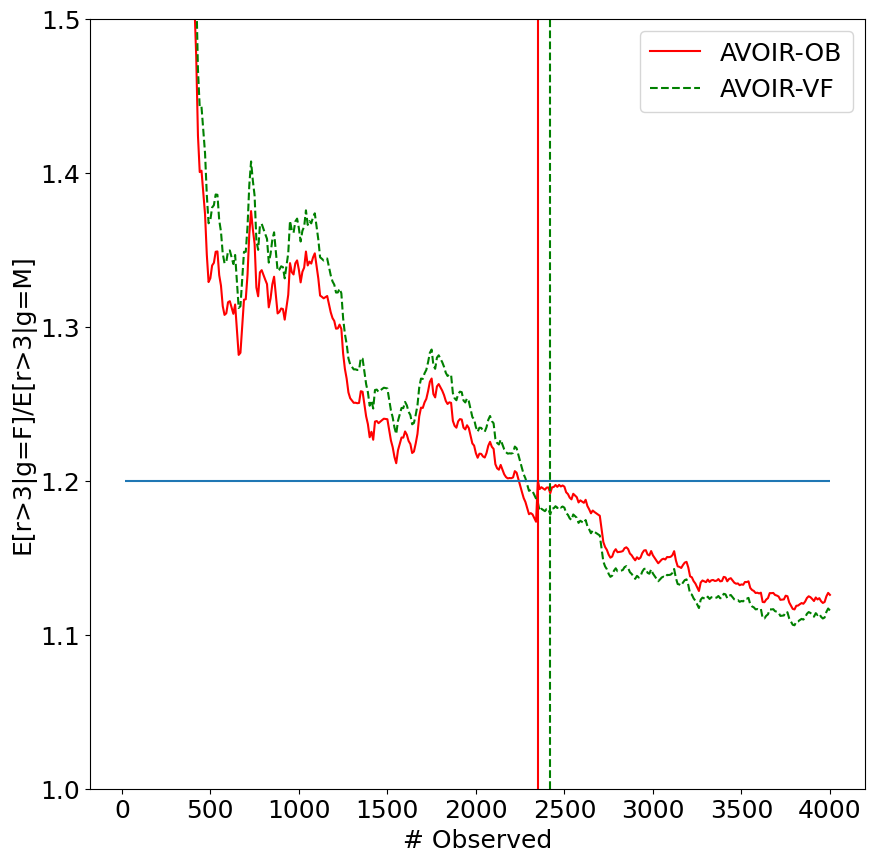
\includegraphics[width=\linewidth]{avoir/images/ratemyprofs.png}
        \caption{Bounds for first half of a gender-fairness specification generated by \AVOIRmethodname{}-OB and AVOIR-VF.}
        \label{fig:casestudy:rmp}
    \end{subfigure}
    \caption{\figleft{} \AVOIRmethodname{} finds a solution for a \textit{theoretical} scenario with $\delta_X + \delta_Y \leq \Delta$ under constraint $\epsilon_X + \epsilon_Y \leq \epsilon_T$ \figright{} For \textit{RateMyProfs}, a real-world dataset, the vertical lines show the step at which the methods can provide a guarantee of failure for the upper bounds with $\Delta <= 0.05$.}
    \label{fig:real-and-theoretical-examples}
\end{figure}


We demonstrate the improvements possible using our approach by instantiating this example with data. 
Suppose we want the upper bound of the failure probability $\Delta = 0.1$ for the specification.
Consider a set of observations such that $\BarE[X] = 0.8, n_X = 1550$ and $\BarE[Y] = 0.5, n_Y = 310$.
Figure~\ref{fig:theoretical-example} shows that no solution is feasible for the optimization problem with $A_\delta$.
However, \AVOIRmethodname{} can find a solution.
For the optimal solution, $\delta_2 \approx 2.35\delta_1$, which aligns with our intuition from section~\ref{sec:related} about allocating higher failure probability to terms with the majority of observations. 
The optimization problem inferred by \AVOIRmethodname{}:
\begin{align}
    \begin{split}
        &\min\limits_{\delta_X, \delta_Y}{\delta_X + \delta_Y} \\
        \text{s.t.  } &\epsilon_X + \epsilon_Y \leq \BarE[X] - \BarE[Y] - \epsilon_T \\
        &0\leq \delta_{X,Y} \leq 1
    \end{split}
\end{align}

%\pmcomment{Please point reader to location in appendix on proof.}


 

\begin{comment}
$\Pr[X] - \Pr[Y]  < \epsilon_T$. 
As $\Pr[X] = \E[X]$ for a Bernoulli r.v., this can be simplified as:
\begin{align*}
    \Pr[\Pr[X] - \Pr[Y] < \epsilon_T] &= \Pr[\E[X] - \E[Y] < \epsilon_T] \\
                                  &= 1 - \Pr[\E[X] - \E[Y] \geq \epsilon_T] \\
\end{align*}

Suppose $\BarE[X]_{(\epsilon_X, \delta_X)}$ and $\BarE[Y]_{(\epsilon_Y, \delta_Y)}$ be statistical guarantees derived for $X$ and $Y$ respectively. 
From the inference rules in Figure~\ref{fig:inference}, we have 
\begin{align*}
    \Pr[|(\E[X]-\E[Y]) - (\BarE[X] - \BarE[Y])| \geq \epsilon_X + \epsilon_Y] &\leq \delta_X + \delta_Y\\
    \implies \Pr[(\E[X]-\E[Y]) \geq \BarE[X] - \BarE[Y] -  (\epsilon_X + \epsilon_Y)] &\leq \delta_X + \delta_Y \\
    \implies \Pr[(\E[X]-\E[Y]) \geq \epsilon_T] &\leq \delta_X + \delta_Y
\end{align*}
where the last inequality follows if $\BarE[X] - \BarE[Y] - (\epsilon_X + \epsilon_Y) \geq \epsilon_T$
\end{comment}


%\pmcomment{TODO: replace the screenshot with a vector graphic from tikz}

\subsection{Visualization for Interactive Refinement}
Using our specification framework as a backend, we built an interactive application for analysis and refinement of specifications provided in our grammar.
Specifically, fairness specifications can be naturally parsed into a tree because of the structure of the grammar.
Each node of the tree represents some sub-expression in the syntax tree of the overall specification.
These nodes allow a user of \AVOIRmethodname{} to interactively audit and tune the specification definition.
To create the visualization, we use Vega~\citep{satyanarayan2015reactive}, a declarative JSON-based visualization grammar.
%To provide the evaluation plots, we need the evaluation values and the observations that they occurred at.
We log the estimates during runs of \AVOIRmethodname{} and then output the grammar in a tabular JSON-format that contains a row for each grammar element and its associated evaluations.
This tabular data is used by our Vega specification to produce the visualizations.
By selecting one of the nodes in the syntax tree, a user can see a plot of the evaluation values associated with the selected grammar element.
This allows for comparison of multiple grammar elements.
The ability to analyze and compare these evaluation values provides context surrounding specification violations, and assists the user in interacting with and deciding how to refine a specification
We provide a detailed example of how these interactions can help \AVOIRmethodname{} users choose an appropriate fairness metric in Section~\ref{sec:casestudy}.
%Given a user provided machine learning model, dataset, and specification the application simulates a stream of observations to the provided model.
%Following the simulation, a visualization is provided that represents the specification as a syntax tree where each node of the tree corresponds to an element of our grammar.
%Figures \ref{fig:casestudy:boston} and \ref{fig:casestudy:adult} show the visualization.
%Note that for each observation made by our machine learning model, the specification is evaluated to check for violations.
%Each grammar element that makes up the specification is evaluated as well, and thus each grammar element is associated with the value it evaluates to for a given observation.
%For the top level specification, \texttt{<spec>}, there is a boolean value associated with each observation, whereas an expectation term, \texttt{<ETerm>}, is associated with a real value.
%We call these plots evaluation plots and two can be observed at a time (see the plots on the right of figure \ref{fig:casestudy:boston}), each with shared scales along the horizontal axis which denotes observations over time.
%The case studies in section \ref{sec:casestudy} demonstrate the usefulness of the context provided by these visualizations.
%To create the visualization, we use Vega \cite{vega}, a declarative JSON-based visualization grammar.
%To provide the evaluation plots, we need the evaluation values and the observations that they occurred at.
%We log these values during the simulation our application runs, and then output the grammar in a tabular JSON-format that contains a row for each grammar element and it's associated evaluations.
%This tabular data is used by our Vega specification to produce the visualizations.
\begin{comment}
The app proceeds in multiple stages,
\begin{enumerate}
    \item First, a user selects a dataset of interest. We built support for two datasets, but our framework is generic enough for any arbitrary csv dataset.
    \item Following this choice, the input variables and output variable for a machine learning model must be specified.
    \item A machine learing model is then selected from a dropdown. We provide support for three models. However, this is for demonstration purposes only - the specification is agnostic to the choice of a machine learning model.
    \item Finally , a specification is input by the user of the app. On the press of a button, the model is trained and then evaluated on the selected dataset. The output monitored by the spec is passed off to the Vega module for further analysis.
\end{enumerate}
\end{comment}
\section{Evaluation}
\label{sec:casestudy}
In this section, we evaluate \AVOIRmethodname{}.variants through three real-world case studies.
Direct comparisons with existing work are impossible since no other work (to our knowledge) facilitates a general-purpose inference engine for online fairness auditing using arbitrary measures.
We can, however, implement VF's~\cite{bastani2019probabilistic} inference rules within \AVOIRmethodname{} (denoted as \AVOIRmethodname{}-VF).
Note that \AVOIRmethodname{}-VF sidesteps the assumptions of having a known data-generating distribution (made possible by \AVOIRmethodname{}'s reliance on confidence sets), making this variation a more practical and efficient algorithm. 
We denote \AVOIRmethodname{}-OB as the implementation that utilizes the abovementioned optimizations. 
Across the studies, the role of chosen threshold probabilities is similar to that of p-values in statistics.
Typical p-values tend to be $0.05$ and $0.1$, which we demonstrate in the RateMyProfs and COMPAS risk assessment study. 
In our case study of prior work~\cite{angwin2016machine}, we stick to the available definitions and thresholds used in the original analysis.
We expect that regulators will set the threshold probabilities on a case-by-case basis, e.g,, $0.15$ for illustration purposes in the adult income study.%, and we provide the adult income study with  $\Delta =0.15$ as an example.

%An important case study on the COMPAS dataset can be found in Appendix~\ref{sec:appendix:additional-case-studies}. 
\subsection{Rate My Profs}
\label{sec:casestudy:rmp}
\begin{figure}
    \centering
    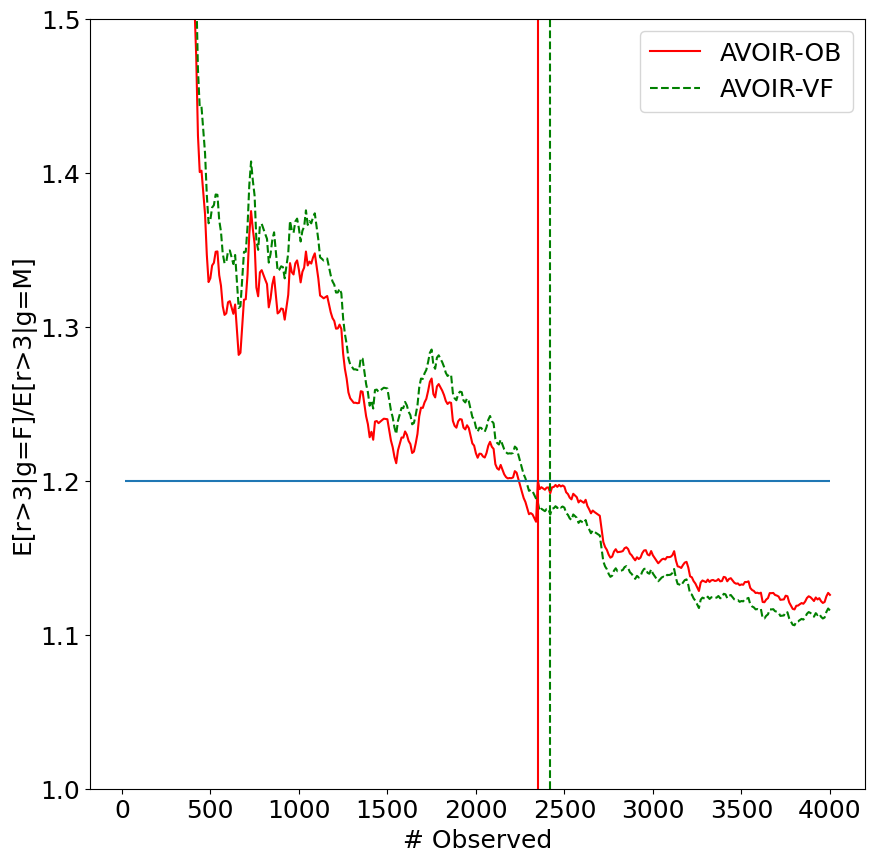
\includegraphics[width=0.5\linewidth]{avoir/images/ratemyprofs.png}
    \caption{Bounds for first half of a gender-fairness specification generated by \AVOIRmethodname{}-OB and \AVOIRmethodname{}-VF for \textit{RateMyProfs}, a real-world dataset. Vertical lines show the step at which the methods can provide a guarantee of failure for the upper bounds with $\Delta <= 0.05$. Blue horizontal line represents the constant term in the inequality.}
    \label{fig:casestudy:rmp}
\end{figure}
This section provides a detailed black-box machine learning model-based case study on a real-world dataset.
This case study uses the Rate My Professors (RMP) dataset~\cite{keymanesh2021fairness}. 
This dataset includes professor names and reviews for them written by students in their classes, ratings, and certain self-reported attributes of the reviewer.
Ratings are provided on a five-point scale (1-5 stars).
We use the preprocessing described in~\cite{keymanesh2021fairness} to infer the gender attribute for the professors.
This dataset is divided into an 80-20 split (train-test).
We then train a BERT-based transformer model~\cite{devlin2019bert} on the training split.
We use the implementation from the simpletransformers\footnote{https://simpletransformers.ai/} package.
The loss function chosen is the mean-squared error from the true ratings.
On the test set, we track a gender-fairness specification in the model outputs:
\begin{lstlisting}[columns=flexible, language=Python, basicstyle=\small]
(E[r > 3 | gender = F] / E[r > 3 | gender = M < 1.2) & 
(E[r > 3 | gender = M)] / E[r > 3 | gender = F] > 0.8)
\end{lstlisting}
We set the failure probability $\Delta = 0.05$. 
\texttt{OPT} is run after each batch (5 items/batch).
Figure~\ref{fig:casestudy:rmp} shows that \AVOIRmethodname{}-OB\footnote{OB = Optimized Bounds} can provide a guarantee in $\mathbf{2.5\%}$ fewer iterations than \AVOIRmethodname{}-VF. 
Note also that the OB guarantee provided tries to optimize for the failure probability while staying under the required threshold, remaining closer to the required threshold in subsequent steps.

\subsection{Adult Income}
\label{sec:casestudy:adult}
In this case study, we analyze the Adult income dataset~\citep{kohavi1996scaling}.
The historical dataset labels individuals from the 1994 census as having a \emph{high-income} ($>50$k a year) or not ($\leq50$k a year).
We consider this column of data as a black-box measurement. 
US Federal laws mandate against race and sex-based discrimination.
Thus, the specification we start our analysis with is a group fairness property for federal employees that monitors the difference of the proportions of individuals with sex marked male vs. female with a high income should be less than $0.5$.
In addition, we ensure that the difference between individuals with race marked white and non-white should have a difference of less than $0.5$.  
Thus, we use an \textit{intersectional} fairness criterion.
The associated specification is given below, where \texttt{h} is an indicator for whether an individual is \emph{high-income} is the binary classification output of our model:

\begin{lstlisting}[columns=flexible, language=Python, basicstyle=\small]
   (E[h | sex=M] - E[h | sex=F] < 0.5) & \ 
   (E[h | race=W] - E[h | race!=W] < 0.5)
\end{lstlisting}

In this example, we set the failure threshold probability $\Delta = 0.15$
\begin{figure}
    \centering
    \begin{subfigure}{0.48\linewidth}
    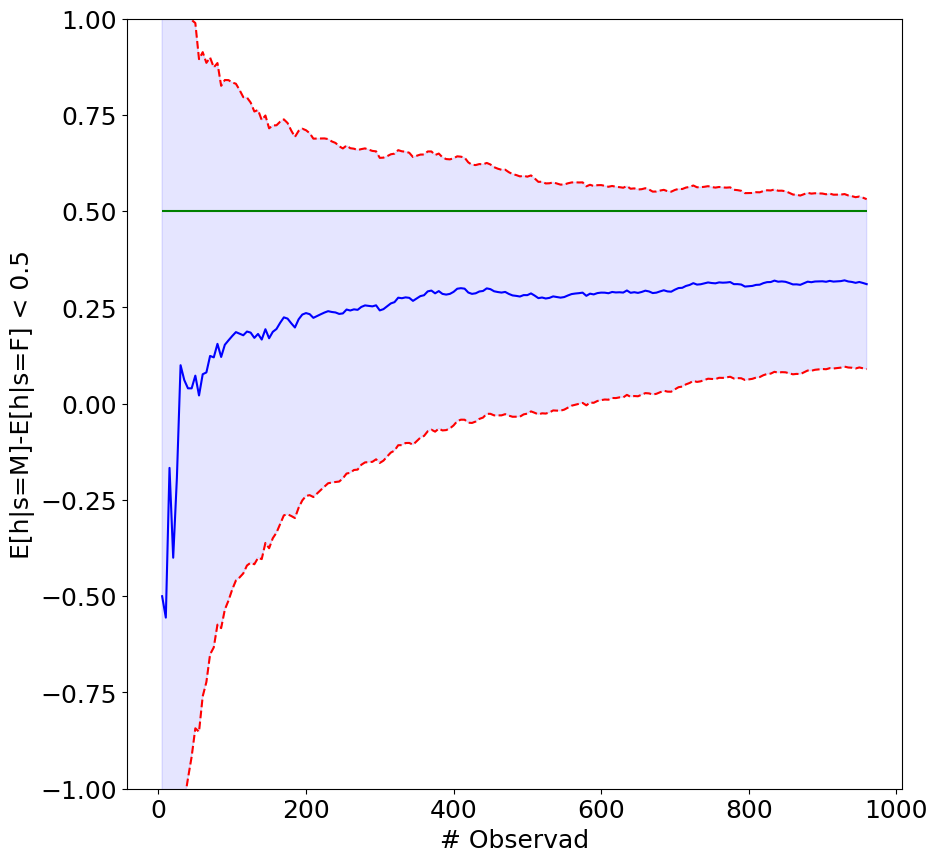
\includegraphics[width=\linewidth]{avoir/images/adult-left-initial.png}
    \caption{Group fairness for sex. Difference in ratio of high income (left subexpression).}
    \label{fig:casestudy:adult:specplot:left}
    \end{subfigure}
    %
    \begin{subfigure}{0.48\linewidth}
    \centering
    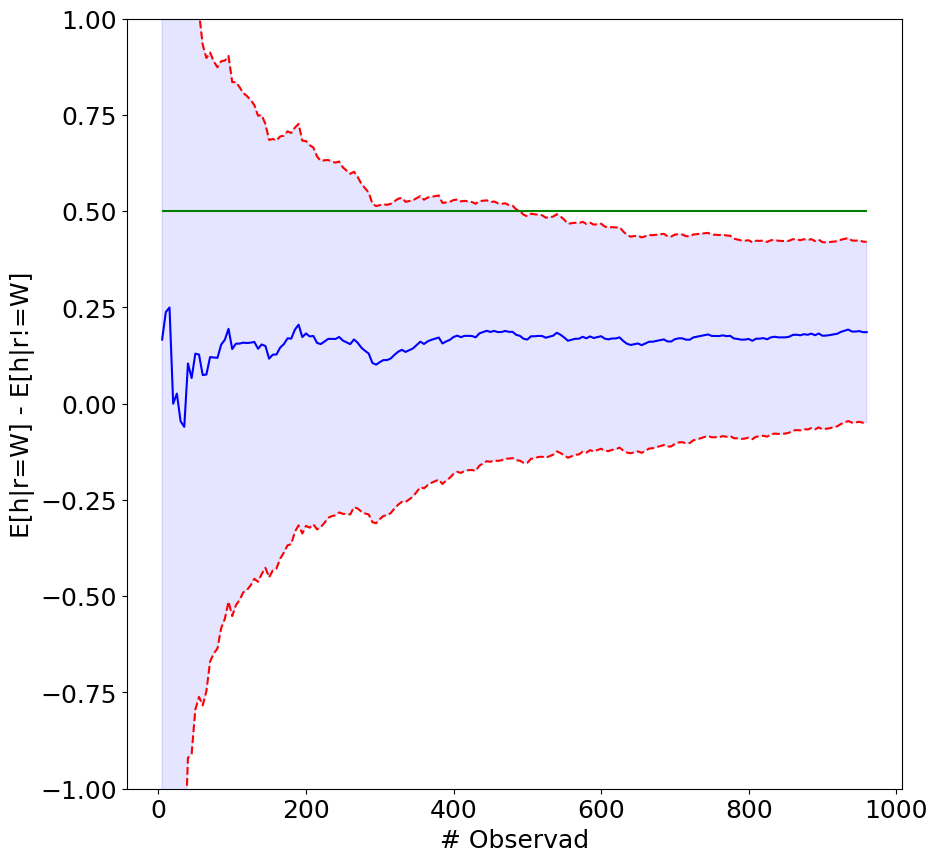
\includegraphics[width=\linewidth]{avoir/images/adult-right-initial.png}
    \caption{Group fairness for race. Difference in ratio of high-income earners (right subexpression). }
    \label{fig:casestudy:adult:specplot:right}
    \end{subfigure}
    \caption{\figtop{} Red dotted lines, the upper bounds of the value cannot be guaranteed to be under the threshold at the specified failure probability. \figbottom{} Guarantee possible with given data. Green lines represent the constant term, and dark blue is the empirical mean.}
\end{figure}
When run with this specification, the generated bounds cannot be achieved with the available data. 
We can then use the iterative refinement associated with subexpressions to analyze different components of the specification. 
The plot corresponding to the left subexpression is shown in Figure~\ref{fig:casestudy:adult:specplot:left} shows that guarantees cannot converge under the threshold with the given number of data samples. 
An auditor can now choose to either reduce the guarantee (i.e. increase $\Delta$) or increase the threshold. 
Next, analyzing the right subexpression, the race group fairness term can be guaranteed to be under the threshold (Figure~\ref{fig:casestudy:adult:specplot:right}).
Using this information, an auditor can make a decision to increase the threshold on the group fairness term for sex. 
As a hypothetical, suppose they increase it from $0.5$ to $0.55$ and rerun the analysis.
OB can provide a guarantee at this threshold within 870 steps, whereas VF can provide it at 960 steps, demonstrating a relative improvement of about $\mathbf{10.35\%}$.
Additionally, the optimal $\Delta$ split across the terms is $\approx (0.135, 0.36 * 10^4)$, which is far from the equal split allocated by VF.
The reason for this split is that increasing the threshold for the first time provides the optimizer with additional legroom to better distribute the failure probabilities between the two terms.

\subsection{COMPAS Risk Assessment}

The Correctional Offender Management Profiling for
Alternative Sanctions (COMPAS) recidivism risk score data is a popular dataset for assessing machine bias of commercial tools used to assess a criminal defendant's likelihood to re-offend.
The data is based on recidivism (re-offending) scores derived from software released by Northpointe and widely used across the United States for making sentencing decisions.
In 2016, \citet{angwin2016machine} at ProPublica released an article and associated analysis code critiquing machine bias associated with race present in the COMPAS risk scores for a set of arrested individuals in Broward County, Florida, over two years.
The analysis concluded that there were significant differences in the risk assessments of African-American and Caucasian individuals.
Northpointe pushed back in a report~\citep{dieterich2016compas} firmly rejecting the claims made by the ProPublica article; instead, they claimed that \citet{angwin2016machine} made several statistical and technical errors in the report.
In this case study, we use \AVOIRmethodname{} to study the claims of the two reports mentioned above. 
%First, we start with the data released by ProPublica and load it into a pandas-simulated DB.
We create a materialized view of the ProPublica dataset by reproducing the preprocessing steps in the publicly available ProPublica analysis  notebook\footnote{https://github.com/propublica/compas-analysis}.
We look at ``Sample A''~\citep{dieterich2016compas}, where the analysis of the ``not low'' risk assessments using a logistic regression model reveals a high coefficient associated with the factor associated with race being African-American.
In terms of a fairness metric, this corresponds to false positive rate (FPR) balance (predictive equality)~\citep{verma2018fairness} metrics. 
The associated specification in \AVOIRmethodname{} grammar would be

\begin{lstlisting}[columns=flexible, language=Python, basicstyle=\small]
   E[hrisk | race=African-American & recid=0] / 
   E[hrisk | race=Caucasian & recid=0] < 1.1
\end{lstlisting}

Where \verb|hrisk| is an indicator for high-risk assessments made by the \emph{black-box} COMPAS tool as defined by ~\citet{angwin2016machine},  \verb|recid| is an indicator for re-offending within two years of first arrest, and a $90\%$-rule is used as the threshold. 
We choose a failure threshold probability of $\Delta = 0.1$, with the optimization run after every batch of $5$ samples.
\AVOIRmethodname{} finds that when the decisions are made sequentially, online, the assertion for specification violation cannot be made with the required failure guarantee.

By analyzing the component subexpressions, one can glean that \AVOIRmethodname{} cannot optimize since the lower FPR in the denominator (FPR for Caucasian individuals) increases the overall variance and limits the ability to optimize for guarantees. 
We follow this analysis by using the reciprocal specification, i.e.,
\begin{lstlisting}[columns=flexible, language=Python, basicstyle=\small]
   E[hrisk | race=Caucasian & recid=0] /
   E[hrisk | race=African-American & recid=0] > 0.9
\end{lstlisting}

We find that the specification is guaranteed to be violated with a confidence of over $1 - \Delta = 0.9$ probability, and \AVOIRmethodname{} can detect this violation within about half the number of available assessments (3350 steps) when run in an online setting.
Figure~\ref{fig:casestudy:compas:propublica} demonstrates the progression of the tracked expectation term. 
Thus, if deployed with the corrected specification, \AVOIRmethodname{} would be able to alert Northpointe/an auditor of a violation/potentially-biased decision-making tool.

\begin{figure}
    \begin{subfigure}{0.48\linewidth}
        \centering
        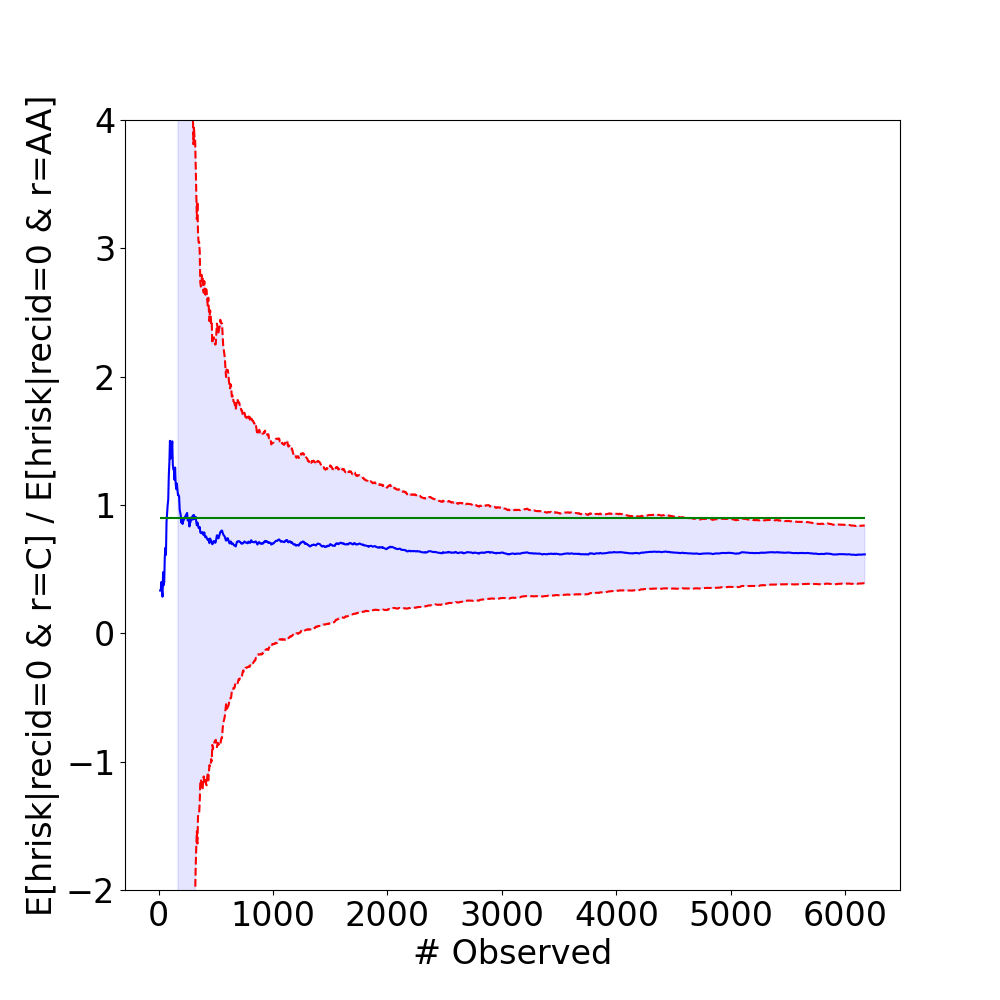
\includegraphics[width=\linewidth]{avoir/images/compas-propublica-et.png}
        \caption{(ProPublica) COMPAS, ``Sample A'' False Positive Rate Bias specification required to \emph{above} the $10\% \implies 0.9$ threshold converges to a value that can be guaranteed to be \emph{under} the required threshold.}
        \label{fig:casestudy:compas:propublica}
    \end{subfigure}
    \hfill
    \begin{subfigure}{0.48\linewidth}
        \centering
        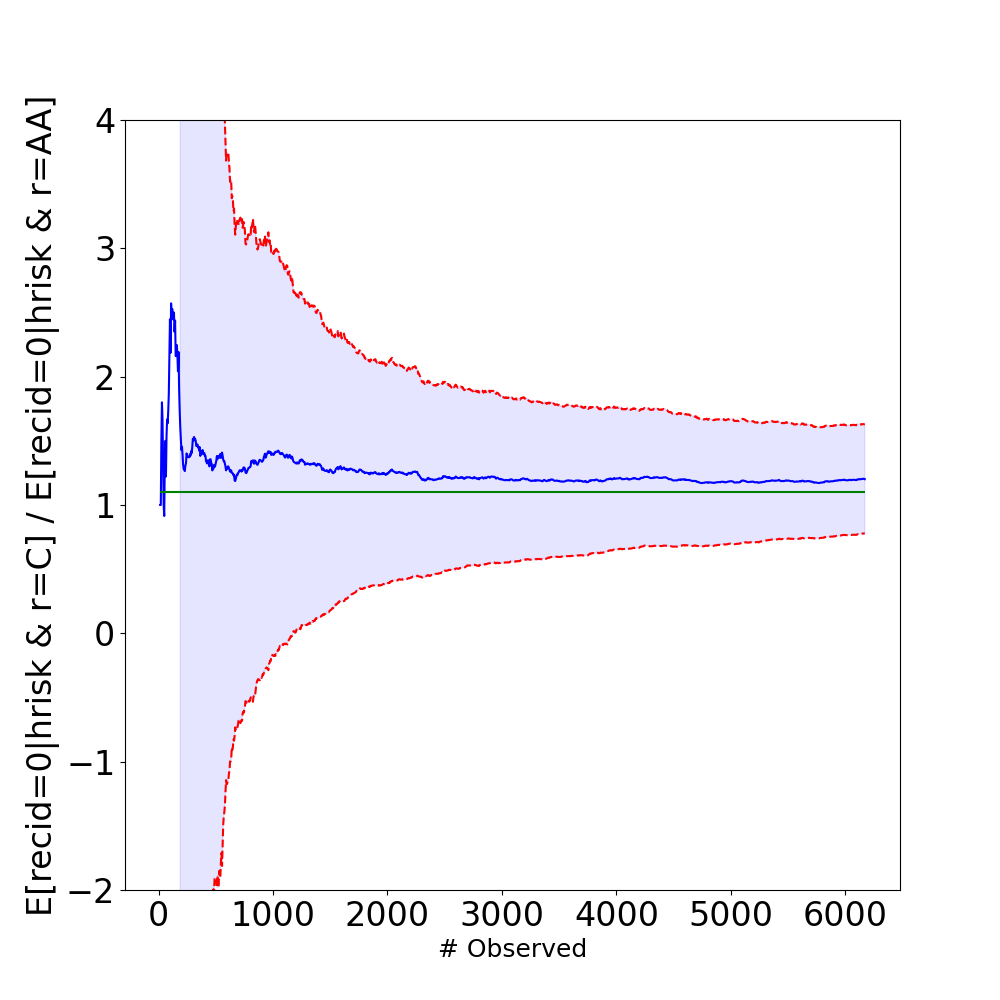
\includegraphics[width=\linewidth]{avoir/images/compas-northpointe-et.png}
        \caption{(Northpointe) ``Sample B'' analysis done by Northpointe using False Discovery Rate that opposed the ProPublica reports.}
        \label{fig:casestudy:compas:northpointe}
    \end{subfigure}
    \caption{COMPAS dataset case study.}
\end{figure}


The Northpointe report~\citep{dieterich2016compas} makes several claims about the shortcomings of this analysis.
One of the primary claims is that \citet{angwin2016machine} used an analysis based on ``Model Errors'' rather than ``Target Population Errors''.
In fairness specification terms, this refers to the difference between a False Positive Rate (FPR) balance vs. False Discovery Rate (FDR) balance, i.e., balancing for predictive parity over predictive equality. 
In probabilistic terms, the difference amounts to comparing $\Pr[\hat{Y} = 1 | Y = 0, g=1, 2]$ (FPR) vs $\Pr[Y = 0 | \hat{Y} = 1, g=1, 2]$ (FDR), where $\hat{Y}$ refers to the decision made by the algorithm, $Y$ refers to the true value, and $g = 1, 2$ reflects group membership~\citep{verma2018fairness}.
This analysis is run on the dataset subset dubbed ``Sample B''.
To test their hypothesis, we reproduce the corresponding preprocessing steps and run both versions (numerator and denominator being Caucasian) of the corresponding specification under the same setup as earlier. 
Despite the point estimate being within the required threshold, we find that neither version can be guaranteed with the required confidence in the given data.
Due to the paucity of space, we describe only one of the two variants with the corresponding figure (Figure~\ref{fig:casestudy:compas:northpointe}).
\begin{lstlisting}[columns=flexible, language=Python]
   E[recid=0 | race=Caucasian & hrisk] /
   E[recid=0 | race=African-American & hrisk] > 0.9
\end{lstlisting}


We note that the Northpointe report~\citep{dieterich2016compas} does not provide confidence intervals for their claim. 
Further, even though the report does not release associated code, the point estimates of the False Discovery Rates (FDRs) match those present in the report, which increases our confidence in our \AVOIRmethodname{}-based analysis. 

The back-and-forth exchange has been the subject of much discussion in academic and journalistic publications~\citep{feller2016computer, washington2018argue}.
Seminal work by \citet{kleinberg2017inherent} proved the impossibility of simultaneously guaranteeing certain combinations of fairness metrics.
While \AVOIRmethodname{} cannot circumvent this problem, its usage can help audit claimed guarantees on defined metrics.
We conclude this case study by noting that \AVOIRmethodname{} lends itself to successful analysis that is not possible with the VF implementation available online, which only provides support for a predefined set of specifications and requires access to a data-generating function.
In addition, we choose $0.1$ as the failure probability because it is one of the thresholds used in \cite{angwin2016machine}.  
We set it to the highest used threshold to allow leeway for the claim by Northpointe.
Even under this lax threshold, the analysis by Northpointe fails.

\section{Discussion} %\& Future Work}
The case studies presented in the previous section demonstrate the ability of our tools to provide vital context when deciding how to refine a model or fairness specification.
Although this contextual information makes decisions easier, it is not always clear how one should alter a specification in light of a violation and its relevant context.
%For example, in case study B, the decision was made that the threshold could be lowered from 2. However, it is not obvious how much we should lower this threshold. Further complicating the matter is the fact that we have options when changing the specification. We can lower the threshold constant (2), or we can add a constant multiplier to the expectation of females with high income.
To assist in these decisions, we are currently examining ways work to suggest edits that are likely to achieve the desired intent of a developer.
Using our visual analysis tool for refinement, we can gather edits from developers and then use that data to learn iterative changes to the syntax tree of the specification.
In addition to improving the usability of our tools for making fairness specification refinements, we also envision a more scalable framework.
Our case studies look at a single model with respect to a single dataset. However, real-world deployment of machine learning often contain many clients with models that may differ.
However, real-world deployment of machine learning often contain many clients with models and datasets that may evolve and drift over time.
We take it as future work to study the efficient monitoring of machine learning behavior with respect to a fairness specification in a distributed context, enabling horizontal scalability.
We believe techniques such as decoupling the observation of data and the reporting results from the monitoring of the results are promising and can lead to the desired scalability.

%\vspace{-0.2in}
\section{Conclusion}

We presented the \AVOIRmethodname{} framework to easily define and monitor fairness specifications online and aid in the refinement of specifications. \AVOIRmethodname{} is easy to integrate within modern database systems but can also serve as a standalone system evaluating whether black-box machine learning models meet specific fairness criteria on specific datasets (including both structured and unstructured data) as described in our case studies.
\AVOIRmethodname{} extends the grammar from Fairness Aware Programming~\cite{albarghouthi2019fairness} with operations that enhance expressiveness.
In addition, we derive probabilistic guarantees that improve the confidence with which specification violations are reported.
Through case studies, we demonstrate that \AVOIRmethodname{} can provide users with insights and context that contribute directly to refinement decisions.
To understand the robustness of \AVOIRmethodname{}, we evaluated it along two dimensions: the data/ML model used and changing parameters (thresholds, fairness definitions).
We demonstrated the robustness of the data/model used by evaluating three datasets of varying domains and types (criminal justice - COMPAS, text classification - RateMyProfs, census data - Adult Income). 
For robustness to the thresholds, we used varying failure probability levels ($0.05$, $0.1$, $0.15$) in our case studies.
Note that any probability thresholds over these values for the corresponding studies would converge in fewer iterations, while lower thresholds would require additional data samples.
Our framework builds the foundation for further improvements in fairness specification, auditing, and verification workflows.
Although contextual information from \AVOIRmethodname{} makes decisions more straightforward, it is not always clear how to alter a specification in light of a violation and its relevant context.

To assist in these decisions, we are currently examining mechanisms that suggest edits that are likely to achieve the desired intent of a model developer.
We plan to extend this work to provide intelligent specification refinement suggestions and support distributed machine learning settings.
In addition to improving the usability of our tools for making fairness specification refinements, we also envision a more scalable framework.
Our case studies looked at a single model with respect to a single dataset. 
However, real-world deployment of machine learning often contains many clients with models and datasets that may evolve and drift over time.
We also expect to examine efficient monitoring of machine learning behavior for a fairness specification in a distributed context, enabling horizontal scalability.
We believe techniques such as decoupling the observation of data and reporting results from monitoring the results are promising and can lead to the desired scalability.
%We also plan to explore the use of \AVOIRmethodname{} for fair ranking problems and tailored database integration.

\newpage \section{Reproducibility}
\label{sec:reproducibility}
To enhance the reproducibility of our work, on the theoretical side, all proofs (with the necessary assumptions) are provided in the appendix. 
Specifically, proofs for the inference engine are in Appendix~\ref{sec:appendix:inference-rules}, and proofs for the correctness of bounds are provided in Appendix~\ref{sec:appendix:confseq}. 
Theorem~\ref{theorem:better-stopping}, which shows how \AVOIRmethodname{} improves over prior work is proved in Appendix~\ref{sec:appendix:optimality}.
To reproduce the results of the case studies in the paper, each case study is encapsulated inside a Jupyter notebook. 
These notebooks are attached along with the source code for \AVOIRmethodname{}.
In addition, all datasets used for generating results for the case studies are also attached in the submitted supplementary documentation.
Finally, the model weights used for the \textit{RateMyProfs} study for exact reproduction are provided in a dropbox folder hosted at  \url{https://www.dropbox.com/sh/n5o4vswnkxv34zr/AABthgLMaYL3MuA0KC39Z1G8a?dl=0}.
\begin{comment}
It is important that the work published in ICLR is reproducible. Authors are strongly encouraged to include a paragraph-long Reproducibility Statement at the end of the main text (before references) to discuss the efforts that have been made to ensure reproducibility. This paragraph should not itself describe details needed for reproducing the results, but rather reference the parts of the main paper, appendix, and supplemental materials that will help with reproducibility. For example, for novel models or algorithms, a link to a anonymous downloadable source code can be submitted as supplementary materials; for theoretical results, clear explanations of any assumptions and a complete proof of the claims can be included in the appendix; for any datasets used in the experiments, a complete description of the data processing steps can be provided in the supplementary materials. Each of the above are examples of things that can be referenced in the reproducibility statement. This optional reproducibility statement will not count toward the page limit, but should not be more than 1 page.
\end{comment}
\begin{subappendices}
\section{Inference Rules}
\label{sec:appendix:inference-rules}
In Figure~\ref{fig:inference}, we provide the rules used to determining the constraints and guarantees for a specification.
We represent $ 
X \odot Y : (E, \epsilon, \delta) \equiv \Pr\left(| \E[X] \odot \E[Y] - E | \geq \epsilon \right) \leq \delta
$
where $\odot$ represents a binary operator.
Constraints are represented in $\{ \}$.
%\pmcomment{Need to explain that constraints carry over in missing cases in Figure!\ref{fig:inference}}
%\pmcomment{Add proofs here for inference rules.}
The proof of correctness for each inference rule starts from the assumptions above the horizontal line and derives the assertions below. 
These proofs use ideas similar to those in \cite{bastani2019probabilistic}.
We reproduce the proofs in Appendix~\ref{sec:appendix:constraint:proofs} here for completeness.
%We provide them here for completeness.
Note that the assertions in the base case (elementary subexpressions) can be arrived at by applying $\rm{AIN}$. 

\begin{figure}
\[
\dfrac{X: \left(\BarE[X], \epsilon_X, \delta_X\right), Y: \left(\BarE[Y], \epsilon_Y, \delta_Y\right)}{X \pm Y: \left(\BarE[X] \pm \BarE[Y], \epsilon_X + \epsilon_Y, \delta_X + \delta_Y\right)}
\]
\[
\dfrac{X: \left(\BarE[X], \epsilon_X, \delta_X\right), Y: \left(\BarE[Y], \epsilon_Y, \delta_Y\right)}{ X \times Y: (\BarE[X] \BarE[Y], \epsilon_X \epsilon_Y + \BarE[X] \epsilon_Y + \BarE[Y] \epsilon_X, \delta_X + \delta_Y)} 
\]
\[
\dfrac{X: \left(\BarE, \epsilon, \delta \right), \BarE - \epsilon > 0}{ X^{-1}: \left(\BarE^{-1}, \frac{\epsilon}{\BarE (\BarE - \epsilon)}  , \delta \right)}\text{ (Inverse)} 
\] 
\[
\dfrac{X: \left(\BarE, \epsilon, \delta \right)}{ X^{-1}: \left(\BarE^{-1}, \frac{\epsilon}{\BarE (\BarE - \epsilon)}  , \delta \right), \{ \BarE - \epsilon > 0\}} \text{ (Inverse C)}
\]
\[
\dfrac{X: \left(\BarE, \epsilon, \delta\right), \BarE - \epsilon > c}{ X > c: (T, \delta)} \text{ (True)} \hspace{0.1in} \dfrac{X: \left(\BarE, \epsilon, \delta \right), \BarE  + \epsilon < c}{ X < c: (F, \delta)} \text{ (False)} 
\] 
\[
\dfrac{X: \left(\BarE, \epsilon, \delta\right)}{ X > c: (T, \delta), \{\BarE - \epsilon > c\}} \text{ (True C)} \]
\[
\dfrac{X: \left(\BarE, \epsilon, \delta \right)}{ X < c: (T, \delta), \{\BarE + \epsilon < c\}} \text{ (False C)} 
\] 
\[
\dfrac{\psi_1: (\B_1, \delta_1), \psi_2: (\B_2, \delta_2)}{\psi_1 \wedge \psi_2: (\B_1 \wedge \B_2, \delta_1 + \delta_2)} \text{ (and)} \hspace{0.01in} \dfrac{\psi_1: (\B_1, \delta_1), \psi_2: (\B_2, \delta_2)}{\psi_1 \vee \psi_2: (\B_1 \vee \B_2, \delta_1 + \delta_2)} \text{ (or)}
\]
\[
\dfrac{\psi_1: (\B_1, \delta_1), \{C_{11, \dots, 1k}\}, \psi_2: (\B_2, \delta_2), \{C_{21, \dots, 2m}\}}{\psi_1 \wedge \psi_2: (\B_1 \wedge \B_2, \delta_1 + \delta_2), \{C_{11, \dots, 1k}, C_{21, \dots, 2m}\}} \text{ (and C)} \]
\[
\hspace{0.2in} \dfrac{\psi_1: (\B_1, \delta_1), \{C_{11, \dots, 1k}\}, \psi_2: (\B_2, \delta_2)}{\psi_1 \vee \psi_2: (\B_1 \vee \B_2, \delta_1 + \delta_2),  \{C_{11, \dots, 1k}\} \vee \{C_{21, \dots, 2m}\}} \text{ (or C)}
\]%
\caption{Inference rules used to guarantees for expressions.The inference rules for each compound expression build on the union bound, triangle inequality, and structural induction approach described by \citet{bastani2019probabilistic}. C: Constraint.}
\label{fig:inference}
\end{figure}
\subsection{Inference rules with Constraints}
\label{sec:appendix:constraint:proofs}

%We define guarantees for concentration using an appropriate concentration inequality. 
%Examples are provided in the Appendix~\ref{sec:appendix:inequality}  
%\paragraph{Correctness} 
In Section~\ref{sec:theoretical:propagation} we provided the proofs for $X\pm Y$, $X > c$.
In the following text, we provide the remaining proofs.

\noindent \textit{Product} Starting with $\phi_X, \phi_Y$
%$\phi_X \eqdef (\BarE[X], \epsilon_X, \delta_X)$, $\phi_Y = Y: (\BarE[Y], \epsilon_Y, \delta_Y)$. 
First, from union bound, both of these hold true with probability at least $1 - \delta_X - \delta_Y$.
Then,
{\allowdisplaybreaks
\begin{align*}
|\E[X]| &= |\BarE[X] - \BarE[X] + \E[X]|\\
        &\leq ||\BarE[X]| +  |\BarE[X] + \E[X]| \leq ||\BarE[X]| + \epsilon_X \\
\end{align*}
}
%We have
\begin{align*}
    |\BarE[X]\BarE[Y] &- \E[XY]|  = |\BarE[X]\BarE[Y]  - \E[X]\E[Y]| \\
    %&= |\BarE[X]\BarE[Y] - \BarE[X]\E[Y] + \BarE[X]\E[Y]  - \E[X]\E[Y]| \\
    &= |\BarE[X](\BarE[Y] - \E[Y]) + \E[Y] (\BarE[X]\  - \E[X])| \\
    &\leq |\BarE[X]||(\BarE[Y] - \E[Y])| + |\E[Y]||(\BarE[X]\  - \E[X])| \\
    &\leq |\BarE[X]| \eps_Y + |\E[Y]| \eps_X \\
    &\leq |\BarE[X]| \eps_Y + (|\BarE[Y]| + \eps_Y) \eps_X \\
    &= |\BarE[X]| \eps_Y + |\BarE[Y]| \eps_X + \eps_X \eps_Y
\end{align*}
where the first step follows as $X, Y$ are Bernoulli r.vs.
Therefore, $X \times Y: (\BarE[X] \BarE[Y], \epsilon_X \epsilon_Y + \BarE[X] \epsilon_Y + \BarE[Y] \epsilon_X, \delta_X + \delta_Y)$

\textit{Inverse/Inverse C} Assume $X: \left(\BarE, \epsilon, \delta \right)$ and $\BarE - \epsilon > 0$.
In the constrained case, we start with only the prior assumption. % i.e., $X: \left(\BarE, \epsilon, \delta \right)$
Then,
\begin{align*}
    |\E[X]| &= |\E[X] - \BarE[X] + \BarE[X]| \\
    &\leq |\E[X] - \BarE[X]| + |\BarE[X]| \leq \epsilon_X + |\BarE[X]|
\end{align*}
i.e., $|\E[X]| \leq \epsilon_X + |\BarE[X]|$. 
Also,
\begin{align*}
    |\E[X]^{-1} - \BarE[X]^{-1}| &= \left|\frac{\BarE[X]^{-1} - \E[X]^{-1}}{\BarE[X]  \E[X]^{-1}}\right| \\
    &\leq \frac{\epsilon}{|\E[X]|  |\BarE[X]|} \leq \frac{\epsilon}{|\E[X]| (\E[X] - \epsilon_X)}
\end{align*}
%where the last step follows from the previous derivation and if $\E[X] - \epsilon_X > 0$.
%The latter condition enforces that the sign of the inequality does not change.
VF adds $E[X] - \epsilon_X > 0$ as a precondition; \AVOIRmethodname{} as a post-constraint.
\paragraph{Boolean Operators}
Starting from $\psi_1: (b_1, \delta_1)$, $\psi_2: (b_2, \delta_2)$, we can apply the union bound for $\psi_1 \wedge \psi_2$, $\psi_1 \vee \psi_2$ to derive the rules for and/or.
%\pmcomment{TODO: Complete Proofs}
Similarly, constraints follow the semantics specified by the rules as they also follow from the union bound.




\subsection{Inferred Optimization Problem}
\label{sec:appendix:inferrence-rules:opt}
For a given overall specification $\psi$, suppose $(\epsilon_i, \delta_i$), $i \in \{1, \dots, n\}$ represents the concentration bounds associated with each constituent elementary subexpression. 
Using the inference rules, we can derive the overall $\delta_T = \sum\limits_{i}\delta_i$, along with a set of (say) $K$ constraints 
\[
g_k(\epsilon_{1}, \dots, \epsilon_{n}, \BarE[X_1], \dots, \BarE[X_n]) \leq \epsilon_k
\]
\[
\text{where } \epsilon_k = \left|c_k - \BarE[f(\BarE[X_1], \dots, \BarE[X_n])]\right|
\]
denotes the maximum allowed margin for the $\text{k}^{\text{th}}$ subexpression of form \texttt{<ETerm> <comp-op> c}).
The objective is to minimize the overall failure probability $\delta_T$.
The overall optimization problem can then be formulated as shown in \ref{eq:optimization},
having $n$ optimization variables $\delta_i$ and $2n + K$ constraints (bounds on $\delta_i$ provide the $2n$ constraints).  
A developer using \AVOIRmethodname{} inputs a required acceptable upper bound of failure probability $\Delta$.
If the solution to the optimization problem $\delta_T^* = \sum_i \delta_i \leq \Delta$, then the optimization can conclude with the required confidence in the proved guarantee.
At this point, the developer may choose to terminate \AVOIRmethodname{}.
However, using Corollary~\ref{thm:adaptive-stopping:anytime}, they may continue to run and refine the estimates.

% Metrics table


\section{Concentration bounds}
%Recall the adaptive Hoeffding inequality~\citep{zhao2016adaptive, bastani2019probabilistic} from \Cref{thm:adaptive-stopping}. 

%\AIN*
%\newtheorem{theorem}{Theorem} % TODO: move to my_definitions.tex


Theorem~\ref{thm:adaptive-stopping} provides a mechanism for choosing the stopping time using arbitrary methods for a fixed $\delta$. 
In general, any adaptive concentration inequality suffices; we use $\rm{AIN}_H$ %that does not depend on the empirical variance but is frequently used in scenarios dealing with bounded r.vs.
However, we use confidence intervals to visualize the evolution of sub-expressions (and overall specification) over the sequence of observations. 
To do so, we require an additional result.

\begin{theorem}\cite[Proposition 1, Lemma 1]{zhao2016adaptive}
Let $S_n = \sum_{i=1}^n X_i$ be a random walk from i.i.d. random variables $X_1, \dots, X_t \sim D$. For any $\delta > 0$,
$\Pr[S_\gT \geq f(\gT)] \leq \delta$
for any stopping time $\gT$ if and only if
$\Pr\left[\exists n, S_t \geq f(t) \right] \leq \delta$

\label{thm:zhao:adaptive-hoeffding:anytime}
\end{theorem}

\begin{corollary}
\label{thm:adaptive-stopping:anytime}
For $\delta > 0$, $\Pr[|\BarE_\gT[X] - \E[X]| \leq \epsilon(\delta, \gT)|] \geq 1 - \delta $
for any stopping time $\gT$ if and only if
\[
\Pr\left[\forall t, |\BarE_t[X] - \E[X]| \leq \epsilon(\delta, t)| \right] \geq 1 - \delta
\]
\end{corollary}
%\begin{proof}
%\pmcomment{need to correct this} 
Corollary~\ref{thm:zhao:adaptive-hoeffding:anytime} follows directly from applying Theorem~\ref{thm:zhao:adaptive-hoeffding:anytime} to Theorem~\ref{thm:adaptive-stopping}.
%\end{proof}
Intuitively, Theorem~\ref{thm:adaptive-stopping} holds since we can choose an adversarial stopping rule for $\gT$ that terminates as soon as the boundary for $\epsilon(\delta, t)$ is crossed~\citep{zhao2016adaptive}. 
Thus, when we establish a bound with a stopping rule, %, as long as the underlying distribution remains unchanged,
the bound will hold prior to and after the stopping rule is enforced.
Corollary~\ref{thm:adaptive-stopping:anytime} implies that once we choose an optimal bound for each subexpression, we can extend the bounds derived using Theorem~\ref{thm:adaptive-stopping} to following observations with continued guarantees for subexpressions.
%Note that this does not necessarily imply that the specification will still be True/False with a bounded failure probability since the truth value of the specification depends on the empirical mean.

\subsection{Proof of Theorem~\ref{thm:conf-seq} for Specifications}
\label{sec:thm:conf-seq:proof:contd}

%Recall \Cref{thm:conf-seq}
%\confseq*

Consider any specification $\psi_k$. Let $\psi_k^t : (\hat{b}_{\psi_k}(t), \delta_{\psi_k}(t))$,
where $\hat{b}_{\psi_k}(t) \subseteq \{T, F\}$ is the inferred value and $\delta_{\psi_k}(t)$ corresponds to the confidence for the assertion at time $t$. 
Let the \textit{elementary} subexpressions involved be $X_{k_1}, \dots, X_{k_D}$ corresponding to the index multiset $\etB_k = \{\{k_1, \dots, k_D \}\}$.
Denote $b_{\psi_k}$ as the true value of $\psi_k$, and $\delta_{\psi_k}$ as the inferred threshold at stopping time $\gT$.
From $\rm{INFER}$, we have
\begin{equation}
\hat{b}_k(t), \delta_{\psi_k}(t) = \rm{INFER}(\phi^t_{X_{k_1}}, \dots, \phi^t_{X_{k_D}})
\label{eqn:conf-seq:compound:inf2}
\end{equation}
\begin{align*}
     \Pr[&\exists t \geq 1, b_k \not\in \hat{b}_k(T)]\\
        &\leq \Pr\left[\bigcup\limits_{i = 1}^{D} \exists t \geq 1,  \neg \phi_{X_{k_i}}^t \right]  & \text{ (From \ref{eqn:conf-seq:compound:inf2})} \\
      &\leq \sum\limits_{i\in \etB_k}\Pr\left[\exists t \geq 1, \neg \phi^t_{X_{k_i}}\right]  & \text{ (union bound)} \\
      &= \sum\limits_{i\in \etB_j}\Pr\left[\exists t \geq 1, |\BarE_t[X_{k_i}] - \E_t[X_{k_i}| > \epsilon_{X_{k_i}}(t)\right]  \\
      %& \text{(definition of $\phi^t_{X_{k_i}}$ )} \\
      &\leq \sum\limits_{i\in \etB_j} \delta_{X_{k_i}} & \text{(elementary subexpressions)} \\
      &\leq \delta_{\psi_k}  & \text{ (applying \ref{eqn:conf-seq:compound:inf1} for $t = \gT$)}
\end{align*}
Thus, $b_{\psi_k}(t)$ is a $1-\delta_{\psi_k}$ confidence sequence for $b_{\psi_k}$



\section{Termination Criterion for \AVOIRmethodname{}}
\label{sec:appendix:optimality}
%\betterstopping*
\addtocounter{theorem}{-1}
\begin{corollary}
Under mild conditions, \AVOIRmethodname{} terminates in finite steps with an assertion over the required specification.
\label{corollary:termination}
\end{corollary}
\begin{proof}
We know that the stopping time $\gT \leq \gT^+$, the stopping time for \AVOIRmethodname{}.
Thus, \AVOIRmethodname{} would terminate whenever Verifiar can. 
For completeness, we provide the conditions under which Verifair terminates.
Note that $c \in \R$ corresponds to a constant threshold involved in specification, also presented in the grammar and bound proagation rules.
\begin{itemize}
    \item  For every subexpression $C_k$ occurring in the specification such that it is involved in the inverse or inverse constr. rules (i.e., $\BarE[C_k]^{-1}$), $\BarE[C_k] \neq 0$, $C_k \neq 0$
    \item For every subexpression $C_k$ such that it occurs a True/False type inequality (such as $C_k > c$), $\BarE[C_k] \neq c$, $C_k \neq c$
\end{itemize}
\end{proof}


\section{Supported Metrics}
\label{sec:appendix:additional-metrics}
\begin{table}
    \centering
    \small
    \begin{tabular}{lc}
    \toprule
        Metric Name  & Definition/DSL  \\
    \midrule 
      \multirow{2}{*}{Statistical Parity \citep{dwork2012fairness}} & $\Pr[R|S] = \Pr[R|\neg S]$ \\ 
      \cmidrule{2-2}
      & $\E[r|s] / \E[r|!s] < c$ \\
      \midrule
       \multirow{2}{*}{Predictive Parity \citep{chouldechova2017fair}} & $\Pr[Y|R, S] = \Pr[Y|R, S]$ \\ 
       \cmidrule{2-2}
       & $\E[y|r, s] - \E[y|r, s] > c$ \\
       \midrule
       \multirow{2}{*}{Equal Opportunity \citep{hardt2016equality}} & $\Pr[\neg R|Y, S] = \Pr[\neg R|Y, \neg S]$ \\ 
       \cmidrule{2-2}
       & $\E[!r|y, s] - \E[!r|y,!s] < c$ \\
       \midrule
       \multirow{3}{*}{Equalized Odds \citep{hardt2016equality}} & $\Pr[R|Y=i, S] = \Pr[R]Y=i, \neg S]$, $i=0, 1$ \\ 
       \cmidrule{2-2}
       & $(\E[r|y=0, !s] - \E[r|y=0, s] > c_0)\ \&$ \\
       & $(\E[r|y=1, !s] - \E[r|y=1, s] > c_1)$ \\   
      %  & $ & $(\&  $ \\
       % & $i = 0, 1$ & $(\E[d=1|Y=0, G=f] - \E[d=1|Y=0, G=m] > c_2$\\
    \bottomrule
    \end{tabular}
    \caption{Examples of supported metrics.}
    \label{tab:appendix:supported-metrics}
\end{table}

We provide a non-exhaustive list of statistical group-based fairness criteria and show an exact/approximate equivalent in the \AVOIRmethodname{} DSL in Table~\ref{tab:appendix:supported-metrics}.
We use the notation from Table~\ref{tab:definitions}, assuming that the return value $R$ is a Bernoulli r.v.
We assume that the decision function $f$ tracked by \AVOIRmethodname{} as a signature that takes $X, G, Y$ as input and produces $S$ or $d$ as output.
Note that in their python implementation, $=$ would be replaced by \lstinline{==} and $|$ by the \lstinline{given} keyword.
\begin{comment}
\begin{itemize}
    \item[$G$:] Protected or sensitive attribute. For demonstration purposes, we will use the values $m$ and $f$ to denote majority and minorty classes.
    \item[$X$:] Features describing each individual 
    \item[$Y$:] True label for $X$
    \item[$S$:] Probability $\Pr[Y|X, G]$ predicted for a certain class $c$
    \item[$d$:] Predicted decision for $X$, usually derived from $X$
    \item[$c$:] A threshold to test the specification. For ratios based approximations, this would be a number $1 \pm \eps$ for some small $\eps > 0$. For difference based approxiamtions, this number would be some small $\eps > 0$. When multiple terms are present, we use $c_i$ to denote the $i^{\text{th}}$ threshold.
\end{itemize}
\end{comment}

\section{Implementation Details}
We built a python library to create specifications that can be implemented as a decorator over decision functions. 
The front end interactive application was implemented using streamlit\footnote{https://streamlit.io/} and the visualizations were built in Vega~\cite{satyanarayan2015reactive}.
Each term in the DSL is implemented through a corresponding python class.
New input/output observations are monitored to update all the terms in a specification.
Inference for evaluating the value and bounds is carried out via operator overloading in these classes. 
%This is fairly straightforward.
In line with previous work~\citep{albarghouthi2017fairsquare,bastani2019probabilistic,albarghouthi2019fairness} on distributional verification, we use rejection sampling for conditional probability estimation.
%In the remainder of this section, we describe how how each of these components are implemented. Further, we describe the process for computing point estimates and probabilistic confidence intervals for the values computed for different terms within the spec.



% Typical fairness constraints require 
%Figure~\ref{fig:grammar} describes the final grammar of our specification DSL.

\subsection{Visual Analysis}
\label{sec:implementation:vis}
\begin{figure}
    \centering
    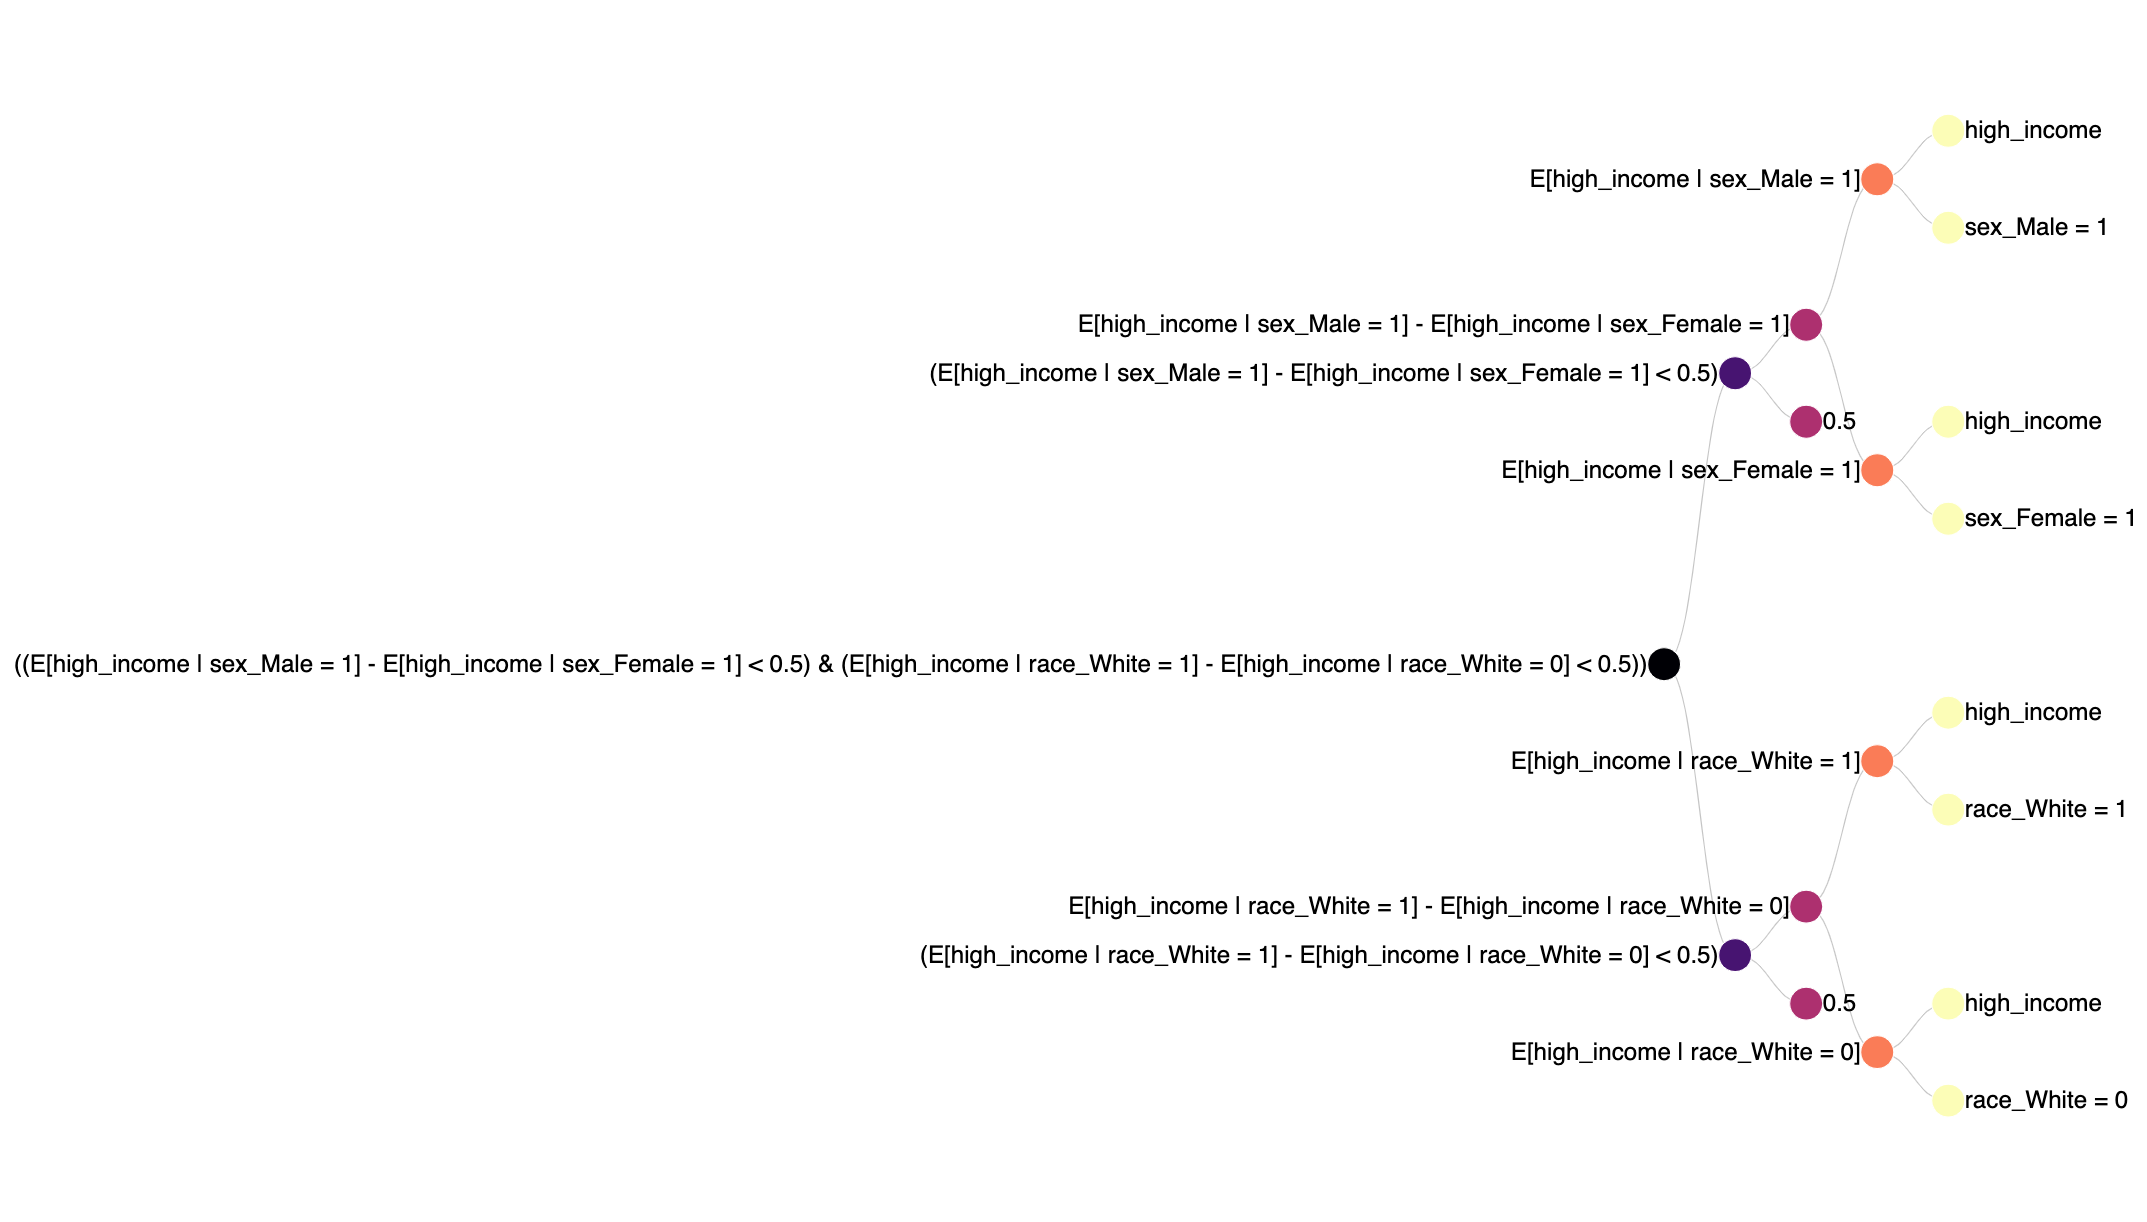
\includegraphics[width=\textwidth, angle=90,alt={Internal representation of parsed tree for a specification.}]{avoir/images/adult-spec-tree-initial.png}
    \caption{Tree corresponding to the initial specification for the Adult Income dataset.}
    \label{fig:impl:adult:initial-spec}
\end{figure}

Using our specification framework as a backend, we built an interactive application for analysis and refinement of specifications provided in our grammar.
Given a user provided machine learning model, dataset, and specification the application simulates a stream of observations to the provided model.
Following the simulation, a visualization is provided that represents the specification as a syntax tree where each node of the tree corresponds to an element of our grammar.
Figure \ref{fig:impl:adult:initial-spec} shows the visualization.

Note that for each observation made by our machine learning model, the specification is evaluated to check for violations.
Each grammar element that makes up the specification is evaluated as well, and thus each grammar element is associated with the value it evaluates to for a given observation.
For specifications \texttt{<spec>}, there is a boolean value associated with each observation, whereas an expectation term, \texttt{<ETerm>}, is associated with a real value.
By selecting one of the nodes in the syntax tree, a user can see a plot of the evaluation values associated with the selected grammar element.
We call these plots evaluation plots and two can be observed at a time 
%(see the plots on the right of figure \ref{fig:casestudy:boston}),
each with shared scales along the horizontal axis which denotes observations over time.
This allows for comparison of multiple grammar elements.
The ability to analyze and compare these evaluation values provides context surrounding specification violations, and assists the user in deciding how to refine a specification.
The case studies in section \ref{sec:casestudy} demonstrate the usefulness of the context provided by these visualizations.

The app for interaction with the backend is built using streamlit. It proceeds in multiple stages,
\begin{enumerate}
    \item First, a user selects a dataset of interest. We built support for four datasets, but our framework is generic enough for any arbitrary csv dataset.
    \item Following this choice, the input variables and output variable for a machine learning model must be specified.
    \item A machine learing model is then selected from a dropdown. We provide support for three models. However, this is for demonstration purposes only - the specification is agnostic to the choice of a machine learning model.
    \item Finally, a specification is input by the user of the app. On the press of a button, the model is trained and then evaluated on the selected dataset. The output monitored by the spec is passed off to the Vega module for further analysis.
\end{enumerate}

\section{AVOIR in Database Setting}

\begin{comment}
\begin{table}
    \centering
    \caption{A summary of the results from the case studies.}
    \label{tab:casestudy:summary}
    \begin{tabular}{ccc}
    \toprule
         Dataset & Setting & Improvement over~\cite{bastani2019probabilistic}  \\
         \midrule
         Adult Income & Database & $10.35\%$ \\
         COMPAS & Materialized View & Interaction\\
         Rate my Profs & ML - BERT & $2.5\%$ \\
         \bottomrule
    \end{tabular}

\end{table}
\end{comment}

In the database literature researchers~\cite{nargesian21tailoring}, have explored an approach to tailoring data integration strategies to ensure that the data set used for analysis has an appropriate representation of relevant (demographic) groups and it meets desired distribution requirements. The authors describe how to acquire such data in an approximate cost-optimal manner for several realistic settings. This work is orthogonal to our work and yet AVOIR can potentially integrate with the authors approach to examine if fairness criteria are being met during the integration process. In other studies on fairness researchers~\cite{yang2018nutritional,asudeh19a,asudeh19b}, have considered the problem of personalized fair ranking functions and discuss approaches to determine if a proposed ranking function satisfies a set of  desired fairness criteria and, if it does not, to suggest modifications that do. AVOIR attempts to solve a  more general purpose problem (not limited to any particular fairness criteria) and is agnostic to the specific model (treats it as a blackbox).  While we have not examined the performance of AVOIR for fair ranking problems, it is something we plan to examine in the future.

To demonstrate how \AVOIRmethodname{} can be integrated within a database system
we use pandas\footnote{https://pandas.pydata.org/} dataframes to simulate the application of \AVOIRmethodname{} in the database setting. 
Specifically, we wrap pandas dataframes with a python `Database' class, and provide a query mechanism to create materialized views.
Queries are provided in the form of python functions that take a dataframe as input and output a corresponding dataframe.
The corresponding view thus generated can be updated with insertion/update/deletion of data.
The specification is added as a decorator inside the refresh function, allowing \AVOIRmethodname{} to track specifications in a database setting.
Note that this tie-in with pandas is only for ease of implementation; the inference engine and optimization can be extended to any database engine.


\end{subappendices}


\endinput